\chapter{Diagrammes de séquence (seq)}
\section{Diagramme de séquence lorsque le locataire entre dans la salle de bain}
Le diagramme ci-après présente l'enchainement des actions en fonction du \textbf{capteur de mouvement Infra-Rouge (IR)}, du contrôleur, du \textbf{radiateur} et des \textbf{éclairages} de la salle de bain.

Le capteur de mouvement IR permet d'indiquer lorsque l'utilisateur entre et sort de la salle de bain. La présence du locataire dans la salle de bain déclenche l'allumage des éclairages et du radiateur si la température intérieure n'est pas assez élevée. A contrario, lorsque l'utilisateur sort de la salle de bain, les éclairages et le radiateur s'éteignent. L'interprétation des mouvements du capteur et le déclenchement des actions sont réalisées au moyen du \textbf{Contrôleur}.

\begin{figure}[H]
	\centering
	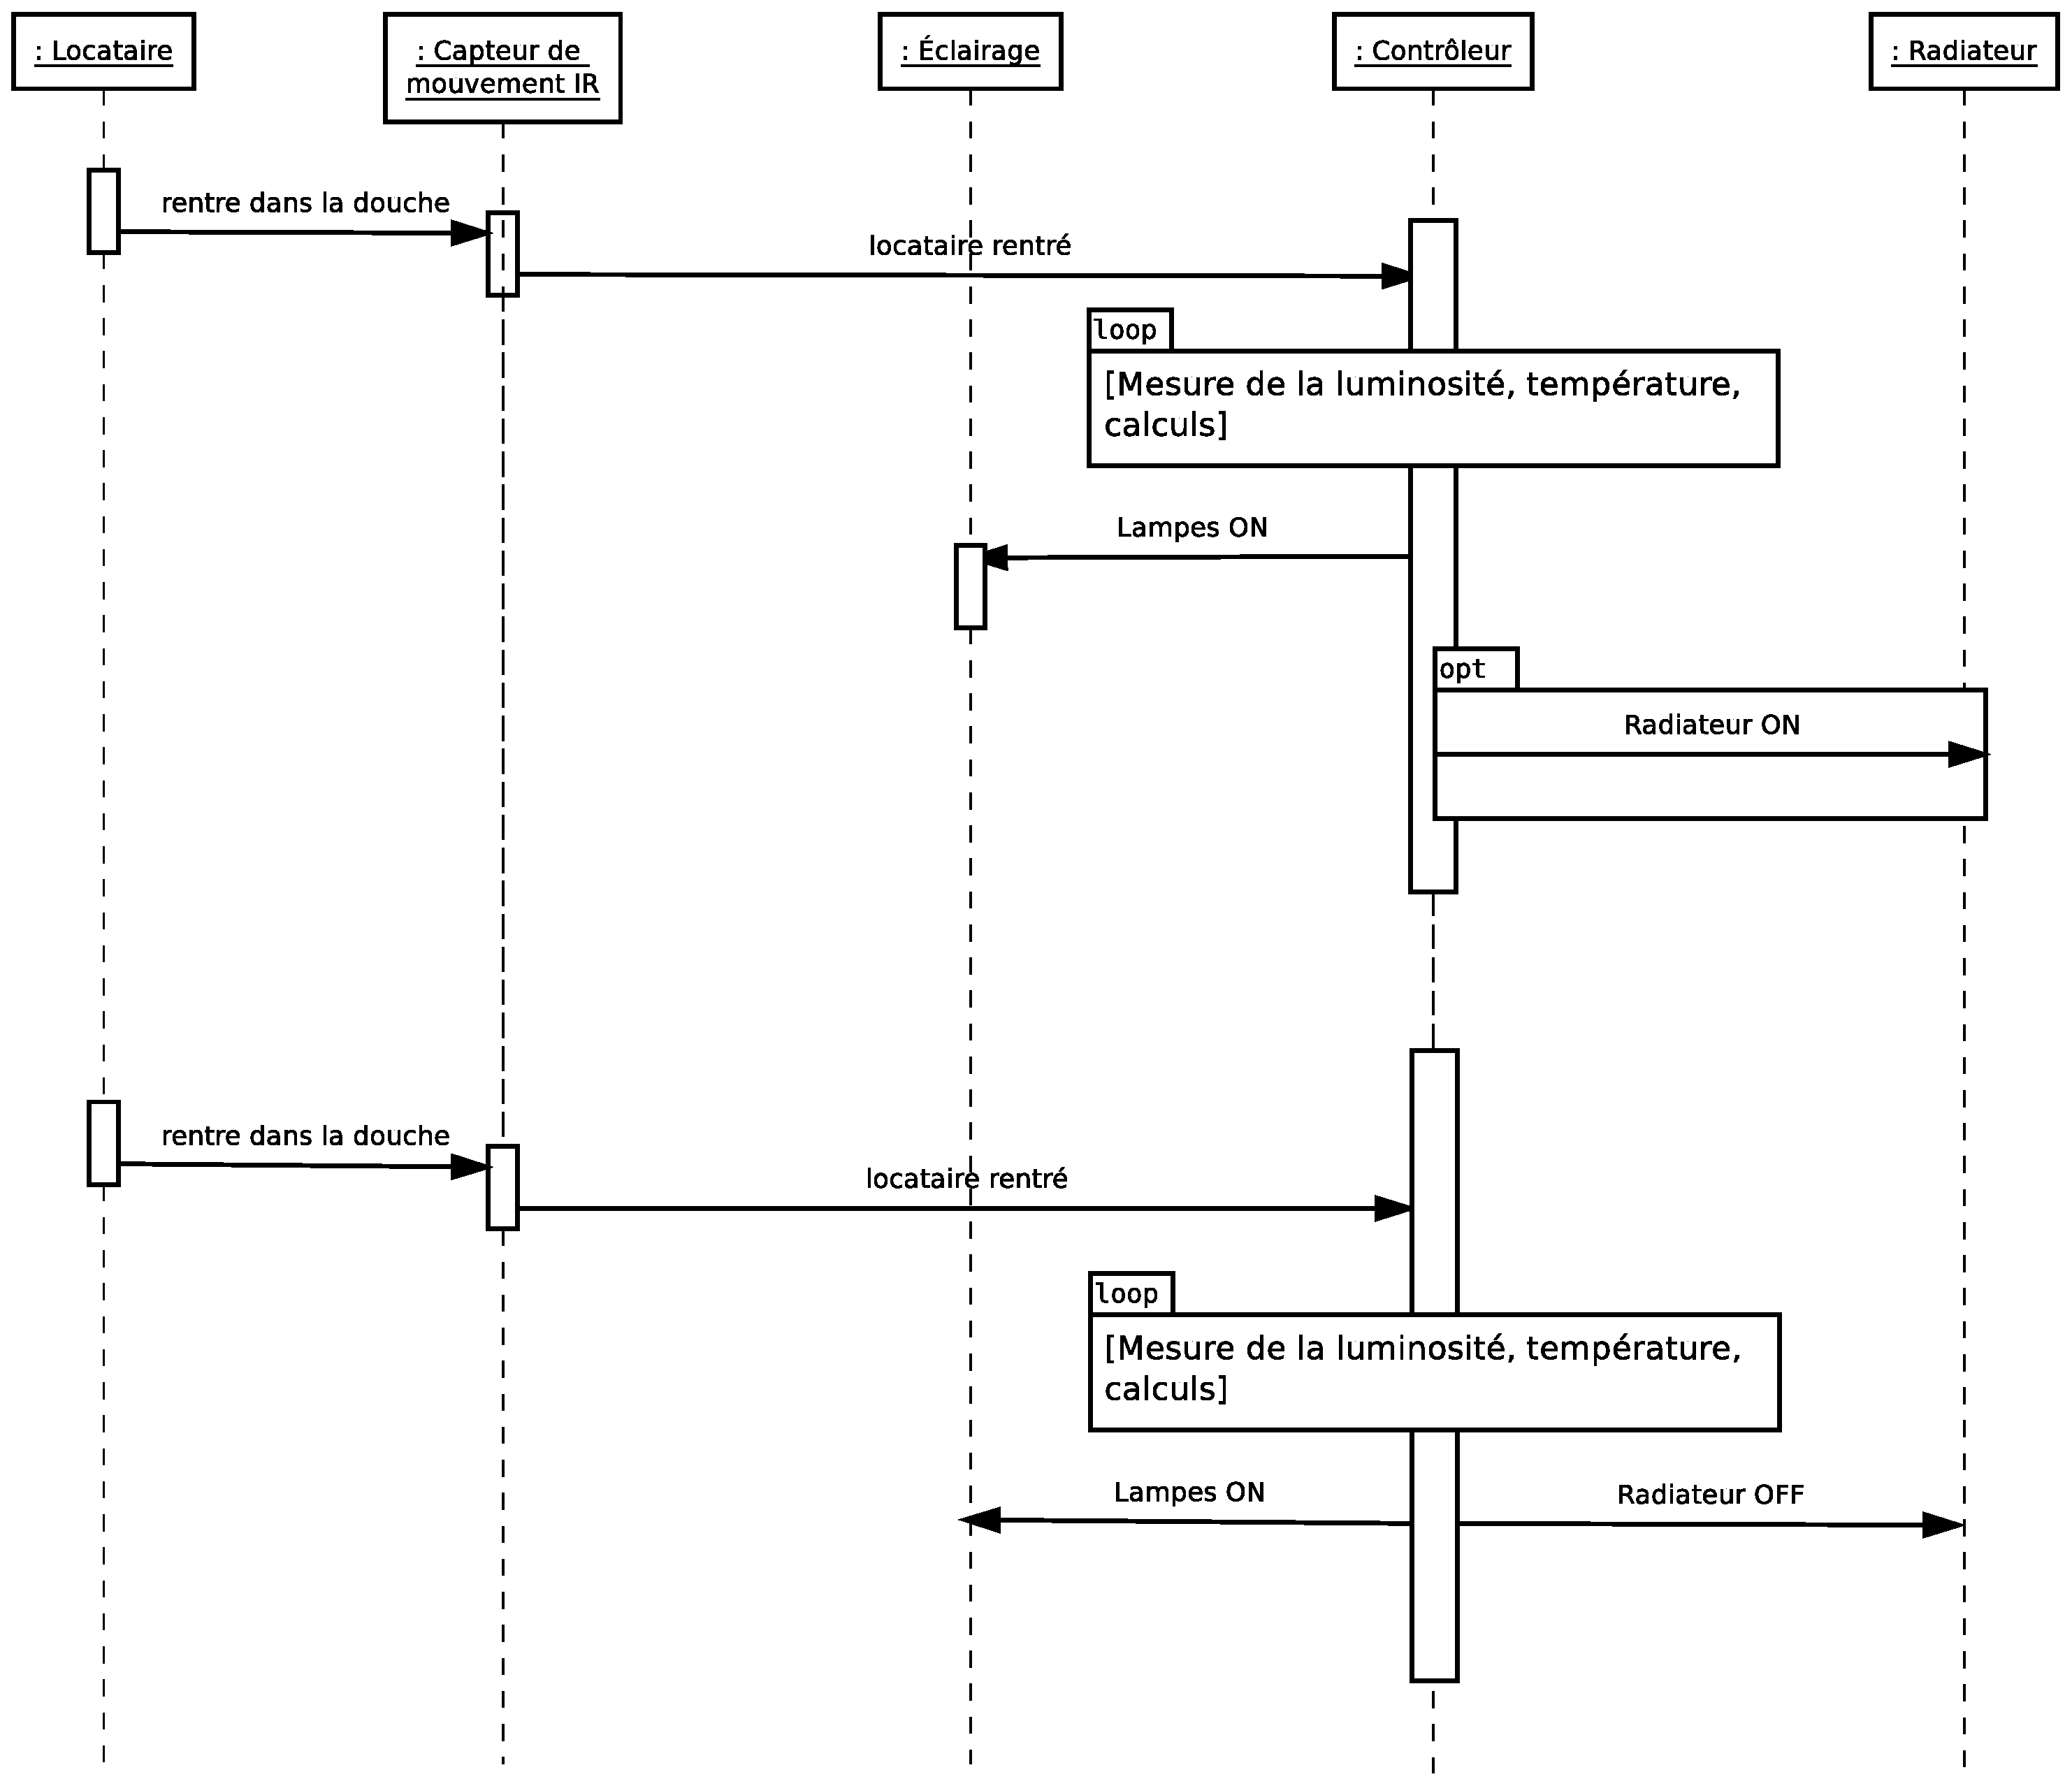
\includegraphics[width=1\linewidth]{diagrams/bathroom/diagramme_sequence.eps}
	\caption{Diagramme de séquence lorsque le locataire entre dans la salle de bain}
	\label{fig:diagramme_seq1}
\end{figure}
\pagebreak

\section{Diagramme de séquence lorsque le locataire entre dans la douche}
Le diagramme ci-dessous présente le déroulement des actions en fonction des différents capteurs (capteur de charge, capteur de position), du contrôleur et de la dalle élévatrice. 

Les capteurs fournissent des informations (présence ou non du locataire dans la douche, hauteur du locataire) qui analyse l'arrivée de ces flux en continu (\textbf{loop}) puis qui procède au traitement afin d'élever ou d'abaisser la dalle élévatrice. 
\begin{figure}[H]
	\centering
	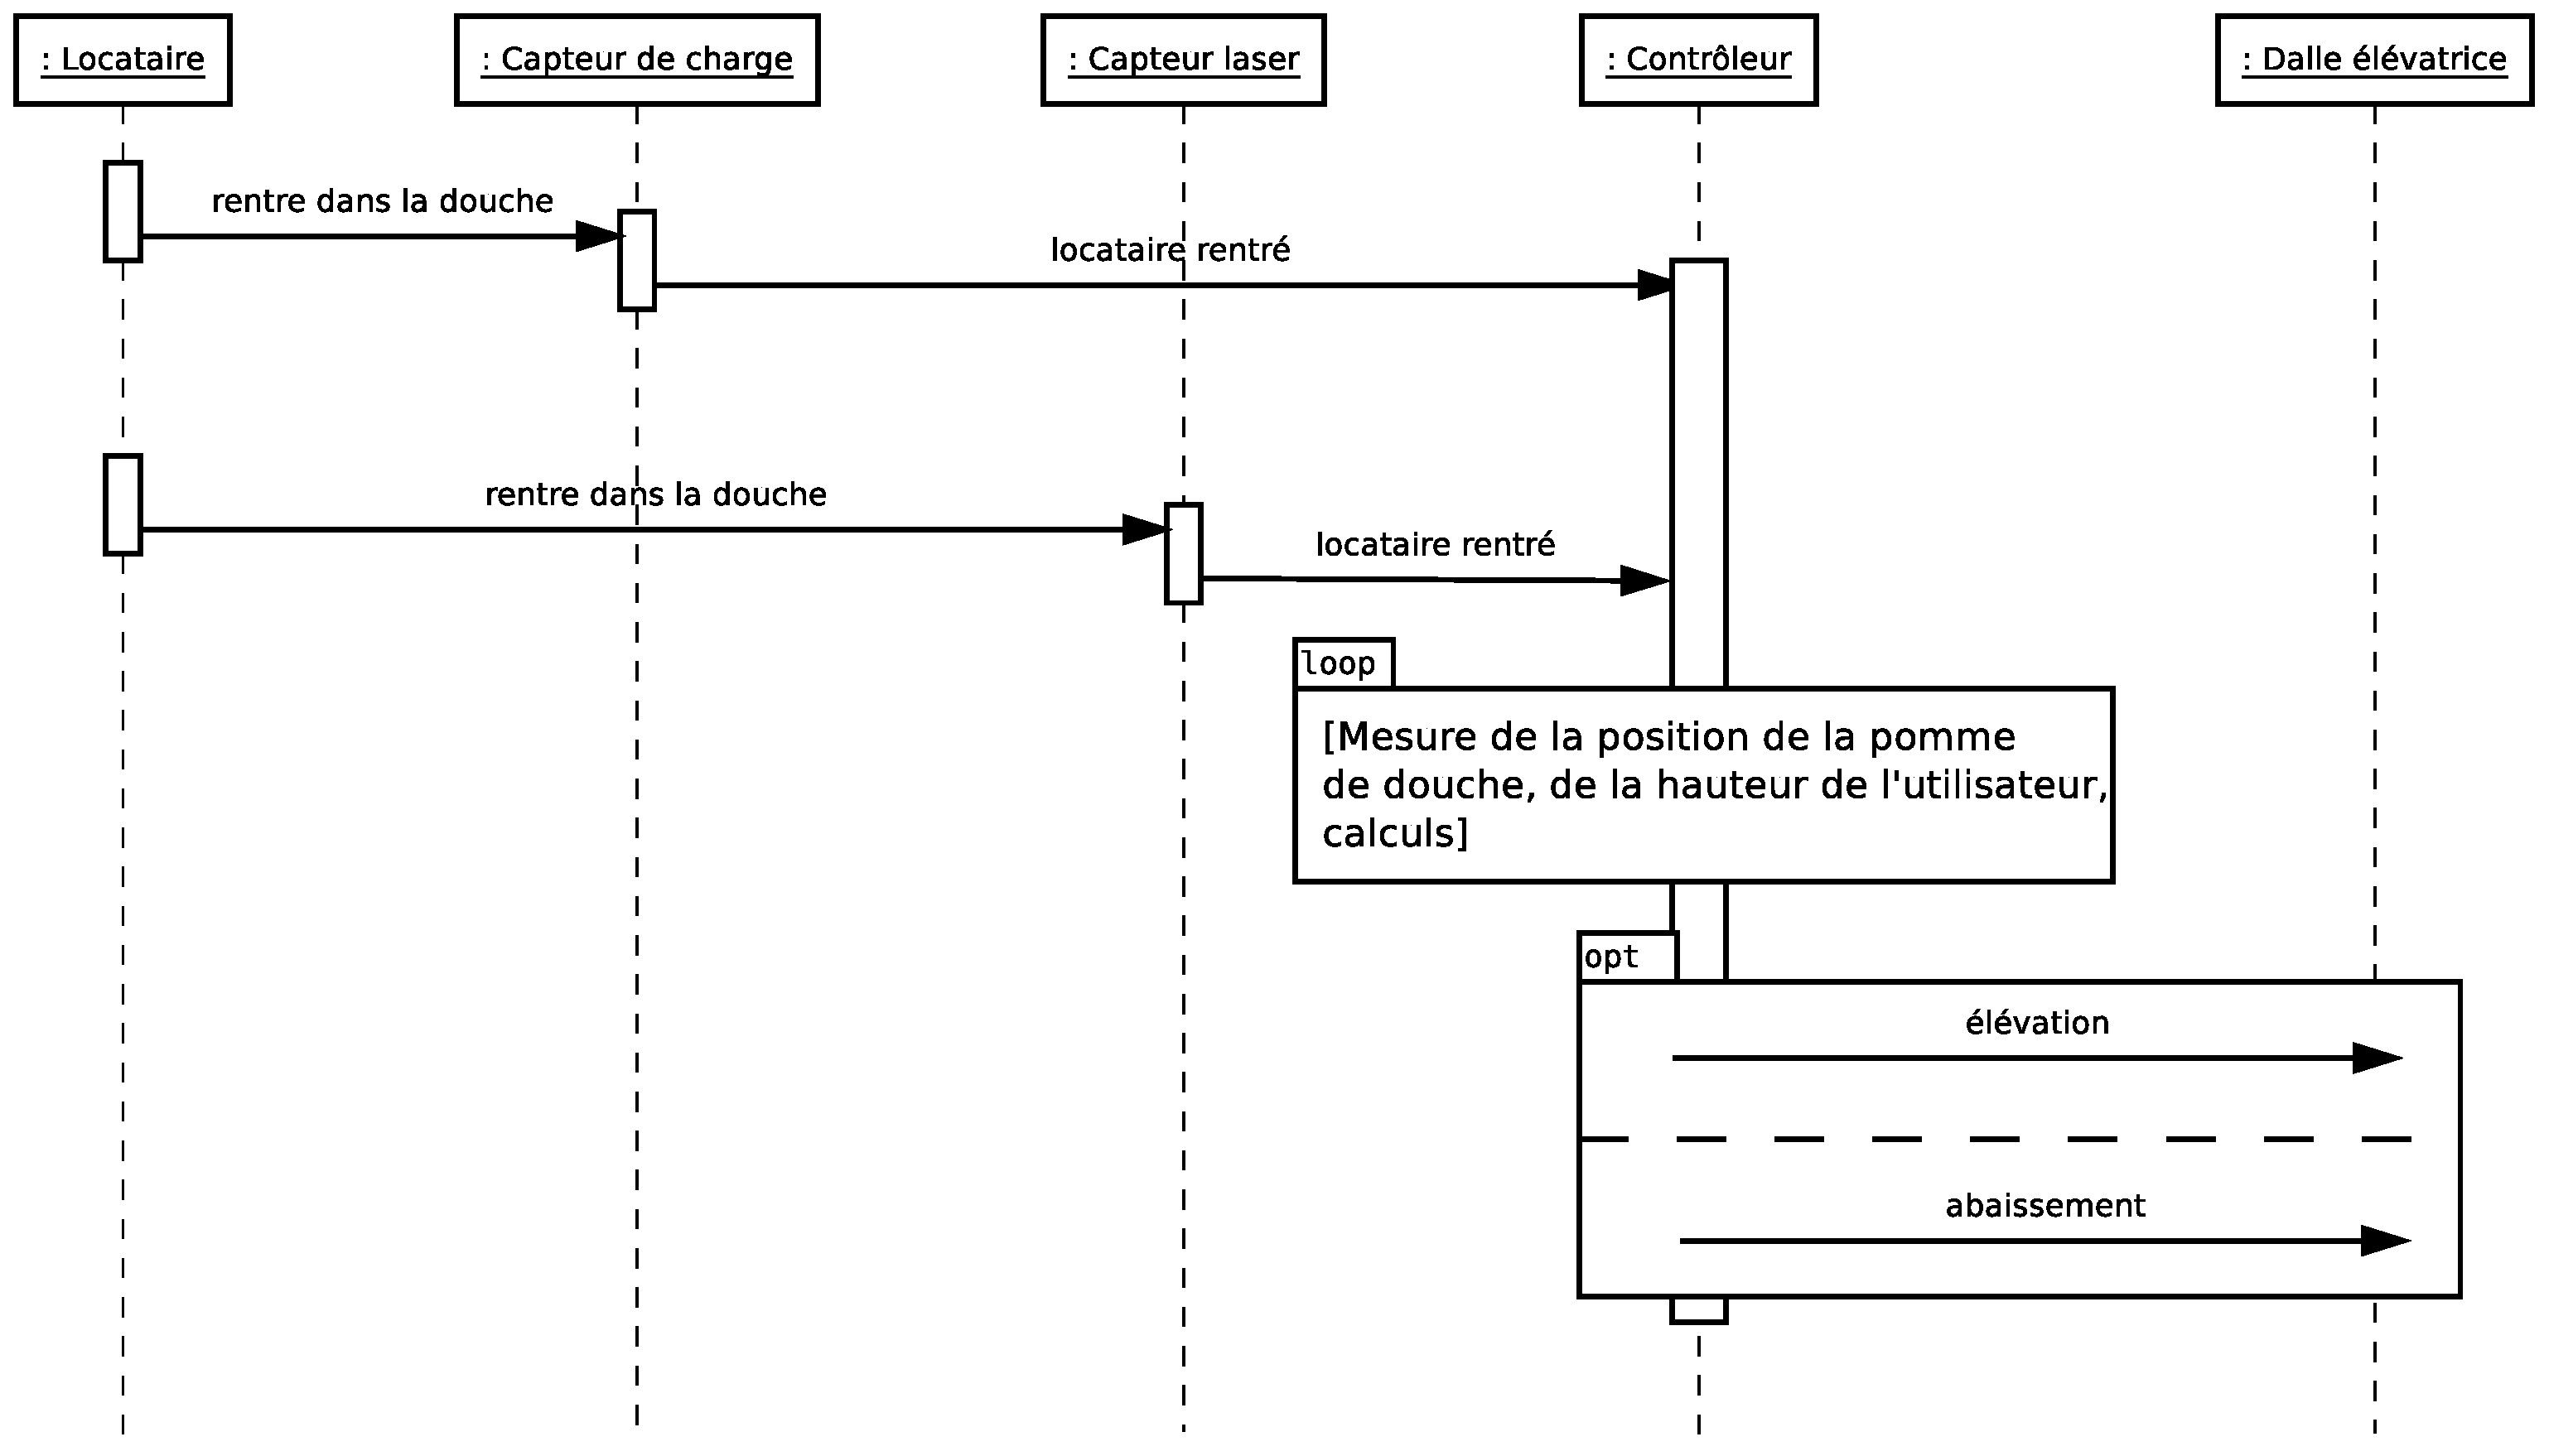
\includegraphics[width=1\linewidth]{diagrams/bathroom/diagramme_sequence2.eps}
	\caption{Diagramme de séquence lorsque le locataire entre dans la douche}
	\label{fig:diagramme_seq2}
\end{figure}
